%%%%%%%%%%%%%%%%%%%%%%%%%%%%%%%%%%%%%%%%%%%%%%%%%%%%%%%%%%%%%%%%%%%%%%%%%%%%
%
%  Template code for the Undergraduate Research Scholars thesis program starting, updated by Undergraduate Research Scholars program staff. Version 6.0. Last Updated: Fall 2024
%  Modified by Tawfik Hussein from the template code for TAMU Theses and Dissertations starting Spring 2018, authored by Sean Zachary Roberson. Version 3.17.09.
%
%
%%%%%%%%%%%%%%%%%%%%%%%%%%%%%%%%%%%%%%%%%%%%%%%%%%%%%%%%%%%%%%%%%%%%%%%%%%%%%%%
%%%%%%%%%%%%%%%%%%%%%%%%%%%%%%%%%%%%%%%%%%%%%%%%%%%%%%%%%%%%%%%%%%%%%%%%%%%%%%%
%%                           SECTION III: RESULTS
%%%%%%%%%%%%%%%%%%%%%%%%%%%%%%%%%%%%%%%%%%%%%%%%%%%%%%%%%%%%%%%%%%%%%%%%%%%%%%%

%_________________(0)______________
% Do not modify. This is the page heading

% THIS LINE PUTS "CHAPTER III RESULTS" AT THE TOP OF THE PAGE, BOLD-FACED AND 14-PT
\chapter{EVALUATION METRICS}

\counterwithout{table}{chapter} % Prevents the table count from resetting in each chapter

\renewcommand*{\thefootnote}{\fnsymbol{footnote}}

\indent\indent To evaluate the performance of the synthesis methods explored in this thesis—AlphaRegex, the L* algorithm, and large language models—we adapted a benchmark suite of 25 regular expression problems originally proposed\footnote{While working with the original benchmarks, we identified an issue in the benchmark examples for task 2 ("Ends with ab"). Specifically, the negative examples did not account for the case where the string consists solely of the character 'b', which does not end with "ab". This oversight could lead to incorrect evaluations of synthesis methods. We updated the benchmark to include this missing negative example, ensuring a more robust evaluation.} in the AlphaRegex paper \cite{lee_2016_synthesizing}. These tasks include string containment, structural alternation, and sequence matching. As shown in Figure~\ref{fig:benchmark-example}, each benchmark begins with a natural language description of the regex problem, followed by a set of positive and negative examples. The benchmarks are loosely organized by increasing difficulty.

\begin{figure}[h!]
	\centering
	Example of a benchmark file used in the evaluation process.
	\begin{verbatim}
	w contains the substring abab
	++
	abab
	XababX
	XXababXX
	--
	a
	b
	XX
	XXX
	XXXa
	XaXX
	bXXX
	XXbX
	\end{verbatim}
	\captionsetup{justification=centering}
	\caption{Example of a benchmark task to find a string that contains "ab". The specificiation starts with a natural language description, followed by positive and negative examples. The "X" in the individual examples represent that this example exists with any character in the alphabet.}
	\label{fig:benchmark-example}
\end{figure}

\begin{table}[h!]
	\centering
	\label{tab:alpha_regex_benchmarks_summary}
	\caption{Summary of the 25 benchmarks, including the number of positive and negative examples, along with the expected human-generated regex solutions.}
	\begin{tabular}{|c|l|c|c|l|}
	\hline
	\textbf{No} & \textbf{Description} & \textbf{Pos} & \textbf{Neg} & \textbf{Human-written} \\
	\hline
	1 & Starts with a & 3 & 3 & $a.*$ \\
	2 & Ends with ab & 3 & 7 & $.*ab$ \\
	3 & Contains the substring abab & 3 & 8 & $.*abab.*$ \\
	4 & Begins with b and ends with a & 3 & 5 & $b.*a$ \\
	5 & Length is at least 3 and the 3rd symbol is a & 3 & 4 & $..a.*$ \\
	6 & Length is a multiple of 3 & 2 & 3 & $(...)*$ \\
	7 & Number of a's is divisible by 3 & 8 & 7 & $(b|(ab*ab*a))*$ \\
	8 & Even number of a's & 7 & 7 & $(b|ab*a)*$ \\
	9 & Fifth symbol from the right is b & 3 & 3 & $.*b....$ \\
	10 & Alternating a and b & 9 & 8 & $b?(ab)*a?$ \\
	11 & Each a in w is followed by at least one b & 7 & 6 & $(b|ab)*$ \\
	12 & a$^n$b$^m$ where $n \geq 3$ and $m$ is even. & 6 & 5 & $aaaa*(bb)*$ \\
	13 & Have at most two a's & 7 & 5 & $b*a?b*a?b*$ \\
	14 & Starting a and odd length or b and even length & 5 & 5 & $a.(..)*|b(..)*$ \\
	15 & Length greater than 1 & 3 & 2 & $...*$ \\
	16 & Does not end with ab & 8 & 3 & $.|.*(a|ba|bb)$ \\
	17 & Contain at least one a and at most one b & 6 & 9 & $a*(ab?|b?a)a*$ \\
	18 & At least two b between any two a & 7 & 7 & $(b*|abbb*a)*$ \\
	19 & Does not contain baa & 8 & 4 & $a*(b|ba)*$ \\
	20 & Every odd position is b & 6 & 9 & $(b.)*b?$ \\
	21 & Consecutive pair aa appears exactly once & 4 & 4 & $(a?b)*aa(ba?)*$ \\
	22 & Length $\ge 2$ and does not end with ba & 9 & 4 & $.*(aa|bb|ab)$ \\
	23 & Even a's, each a is followed by at least one b & 6 & 9 & $(b|abb*ab)*$ \\
	24 & All adjacent a's appear before any adjacent b's & 9 & 9 & $(b?a)*(a?b)*$ \\
	25 & At most one pair of consecutive b's & 5 & 5 & $(b?a)*bb(ab?)*$ \\
	\hline
\end{tabular}
\end{table}



\indent\indent As the different algorithms require different types of input, the evaluation process was tailored accordingly. ChatGPT and AlphaRegex were provided with the benchmark file in its entirety, including the natural language description and examples. For the L* algorithm, the natural language description was interpreted by a human to manually construct the required membership and equivalence queries.

\section{Metrics}

\indent\indent To comprehensively compare synthesis approaches, we defined three categories of evaluation metrics:
Correctness was evaluated by determining whether a solution satisfied all positive examples and rejected all negative examples. Final validation was performed via human inspection to account for edge cases or oversimplified expressions. Efficiency metrics included the number of states explored for AlphaRegex, the number of membership and equivalence queries made for L*, and the wall-clock time required to generate results for all three methods. Complexity was assessed in three ways: total character count, the number of operators, and a subjective readability score ranging from 1 (unreadable) to 5 (clean and intuitive).

\section{Experimental Setup}

\indent\indent We implemented AlphaRegex and L* in Python and the code is readily available as seen in Appendix~A. LLM queries were issued through the OpenAI GPT-4o API (March 2025 snapshot) with a defined system prompt detailing the upcoming inputs.

\chapter{RESULTS AND DISCUSSION}

\indent\indent This chapter presents the results of our empirical evaluation and synthesizes key insights from the behavior of the three synthesis methods studied—AlphaRegex, the L* algorithm, and LLMs. We evaluate these methods on a diverse benchmark suite of 25 regex generation tasks, analyzing their correctness, performance, and complexity across both quantitative and qualitative dimensions.

\section{AlphaRegex Results}

\indent\indent In the original configuration, weights, and heuristics as described in the original paper, the findings indicate that the heuristics do not consistently improve wall-clock time performance as seen in Table~\ref{tab:alpha_regex_performance_seconds}. This is likely due to the overhead associated with verifying solutions against all examples. Specifically, the redundancy elimination heuristic requires significant computational effort, as it involves copying and branching out potential equivalent states, which must then be validated against the entire set of examples. 

\begin{table}[h!]
	\centering
	\caption{Comparison of regex synthesis methods based on wall-clock time. Skipped entries indicate that the algorithm failed to find a solution within the 10,000-second time limit. "Full" refers to the complete process with all heuristics enabled, "No Apr" excludes over-approximation, and "No Rd" disables redundancy elimination. Times are reported in seconds.}
	\label{tab:alpha_regex_performance_seconds}
	\begin{tabular}{|c|p{5cm}|c|c|c|l|}
	\hline
	\textbf{No} & \textbf{Description} & \textbf{Full} & \textbf{No Apr} & \textbf{No Rd} & \textbf{Output} \\
	\hline
	1 & Starts with a & 0.011 & 0.008 & 0.002 & $a.*$ \\
	2 & Ends with ab & 36.06 & 50.96 & 16.99 & $.*ab$ \\
	4 & Begins with b and ends with a & 0.077 & 0.101 & 0.044 & $b.*a$ \\
	5 & Length is at least 3 and the 3rd symbol is a & 0.587 & 0.585 & 0.284 & $..a.*$ \\
	6 & Length is a multiple of 3 & 1.39 & 1.51 & 0.254 & $(...)*$ \\
	8 & Even number of a's & 55.25 & 84.86 & 11.59 & $(b*(ab*a)*)*$ \\
	11 & Each a in w is followed by at least one b & 9.63 & 9.71 & 1.58 & $(b*(.b)*)*$ \\
	15 & Length greater than 1 & 0.058 & 0.0833 & 0.018 & $..*.$ \\
	\hline
\end{tabular}
\end{table}

\indent\indent Additionally, the implementation appears to encounter issues in scenarios requiring union operations. In the cases where the synthesis succeeds, the generated solutions exclusively utilize concatenation and Kleene star operations, with no unions present. This suggests a potential flaw in the implementation when handling union operations.

\begin{table}[h!]
	\centering
	\caption{Performance comparison of regex synthesis methods using the number of states explored/expanded and considered as potential candidate solutions, from the same setup as Table~\ref{tab:alpha_regex_performance_seconds}.}
	\label{tab:alpha_regex_performance_states}
	\begin{tabular}{|c|p{5cm}|c|c|c|}
	\hline
	\textbf{No} & \textbf{Description} & \textbf{Full} & \textbf{No Apr} & \textbf{No Rd} \\
	\hline
	1 & Starts with a & 18 & 23 & 12 \\
	2 & Ends with ab & 20389 & 75483 & 31235 \\
	4 & Begins with b and ends with a & 95 & 238 & 151 \\
	5 & Length is at least 3 and the 3rd symbol is a & 453 & 1195 & 597 \\
	6 & Length is a multiple of 3 & 1143 & 3870 & 487 \\
	8 & Even number of a's & 17124 & 62688 & 17638 \\
	11 & Each a in w is followed by at least one b & 3510 & 17638 & 3105 \\
	15 & Length greater than 1 & 78 & 202 & 3105 \\
	\hline
\end{tabular}
\end{table}

\indent\indent Despite these challenges, the over-approximation and under-approximation heuristics occasionally provide substantial time savings, making their inclusion worthwhile in certain cases. However, when examining the number of states explored in Table~\ref{tab:alpha_regex_performance_states}, the heuristics consistently demonstrate their effectiveness in reducing the search space. They reliably prune unnecessary states and guide the search process in a more efficient direction. This aligns with the findings of the original paper, which reported that while the heuristics were highly effective at limiting the search space, they did not always reduce the time required to find a solution. The overhead introduced by the heuristics could potentially be optimized further in the current implementation to improve overall performance.

\indent\indent AlphaRegex tends to produce regex expressions that are relatively readable, primarily due to its greedy nature in selecting solutions. This approach often prioritizes simplicity and clarity, making the generated regex easier to interpret and understand. However, this same greedy strategy can lead to challenges when dealing with tasks that require deeper nesting or involve ambiguous patterns. In such cases, the algorithm may fail to explore alternative solutions that could better capture the desired behavior. Additionally, the performance and output of AlphaRegex are highly sensitive to the tuning of its weights. Small adjustments to these weights can significantly influence the synthesis process, potentially leading to either improved results or suboptimal solutions. This sensitivity underscores the importance of careful parameter selection to achieve the desired balance between efficiency and correctness.


% \subsection{Weight Analysis}

% \indent\indent We experimented with three different weight configurations to observe how heuristic prioritization changes the generated output. Each configuration emphasizes different regex characteristics: minimal size, reduced use of \texttt{*}, and balanced weight. The results below illustrate how weights impact regex complexity and runtime.

% \indent\indent In the release of the source codes, the weights are set to the default values. The weights are set to the following values:

% TODO 

\section{L* Algorithm Results}

For the initial examples, the majority of proposals tend to default to the empty language. This occurs because the observation table often becomes satisfied and complete once the empty string, single 'a', and single 'b' are all rejected, leading to the conclusion that no strings are accepted.


\begin{table}[h!]
	\centering
	\caption{The results of the benchmarks synthesized by the L* algorithm, demonstrating its performance in generating regular expressions. The Q column refers to the number of membership queries and the P column refers to the number of equivalence queries verifying proposals.}
	\label{tab:l_star_outputs}
		\begin{tabular}{|c|l|c|c|l|}
		\hline
		\textbf{No} & \textbf{Description} & \textbf{Q} & \textbf{P} & \textbf{Output} \\
		\hline
		1 & Starts with a & 14 & 2 & $a.*$ \\
		2 & Ends with ab & 21 & 2 & $b*a(a|bbb*a|ba)*b$ \\
		3 & Contains the substring abab & 29 & 2 & $b*aa*b(aaa*b|bb*aa*b)*ab.*$ \\
		4 & Begins with b and ends with a & 27 & 3 & $bb*a(bb*a|a)*$ \\
		5 & Len $\ge$ 3 and 3rd symbol is a & 44 & 3 & $..a.*$ \\
		6 & Len $\% 3 = 0$ & 17 & 2 & $(...)*$ \\
		7 & Number of a's is divisible by 3 & 14 & 2 & $(b|ab*ab*a)*$ \\
		8 & Even number of a's & 5 & 1 & $(b*a(ab*a|b)*ab*|b*)$ \\
		% 9 & Fifth symbol from the right is b & - & - & $.*b....$ \\
		% 10 & Alternating a and b & - & - & $(ab)*(a)?|(ba)*(b)?$ \\
		% 11 & Each a followed by least one b & - & - & $(b|ba)*$ \\
		% 12 & a$^n$b$^m$ where $n \geq 3$ and $m$ is even. & - & - & $aaa.*(bb)*$ \\
		% 13 & Have at most two a's & - & - & $b*|b*ab*|b*ab*ab*$ \\
		% 14 & Start a odd len or b even len & - & - & $a(..)* | b(..)*$ \\
		% 15 & Length greater than 1 & 20 & 4 & $..*$ \\
		% 16 & Does not end with ab & 38 & 8 & $?|.|.*(aa|ba|bb)$ \\
		% 17 & Contain $\ge$ 1 of a and $\le$ 1 of b & 33 & 7 & $aa*|aa*ba*|a*baa*$ \\
		% 18 & At least two b between any two a & 42 & 9 & $b*a(bb*a)*b*$ \\
		% 19 & Does not contain baa & 36 & 8 & $(aa|ab|ba?|bb)*a?$ \\
		% 20 & Every odd position is b & 29 & 6 & $(b.)*b?$ \\
		% 21 & aa appears exactly once & 48 & 10 & $(b|ab)*aa(b|ab)*$ \\
		% 22 & Length $\ge 2$ and end is not ba & 31 & 7 & $.*(aa|bb|ab)$ \\
		% 23 & Even a's, each a has $\ge$ 1 of b & 39 & 8 & $b*(abb*abb*)*b*$ \\
		% 24 & adjacent $a$'s then adjacent $b$'s & 44 & 9 & $(a|ba)*(bb(a|b)*a?b*)?$ \\
		% 25 & At most one pair of consecutive b's & 46 & 10 & $(a|ba)* | (a|ba)*bb(a|ba)*$ \\
		\hline
	\end{tabular}
	\end{table}

The L* algorithm generates minimal DFAs, though these do not always correspond to minimal regex, especially when guided by specific counterexamples. Its effectiveness is highly dependent on the quality of the teacher, as the teacher provides membership and equivalence queries to refine the DFA. This approach is best suited for simpler patterns or cases where the teacher can provide precise and consistent feedback.

\begin{figure}[h!]
	\centering
	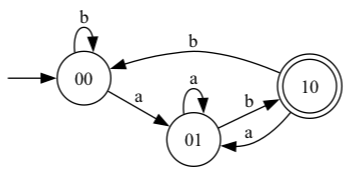
\includegraphics[width=9cm]{figures/ends_with_ab.png}
	\caption{The solution DFA machine to capture a string that ends with ab.}
	\label{fig:ends_with_ab}
\end{figure}

The second example, as shown in Figure~\ref{fig:ends_with_ab}, demonstrates a straightforward DFA. However, the resulting regex is unexpectedly long and complex. This is due to the collapsing process of the DFA and the methodology used to derive the regex, as discussed earlier. Similarly, Figure~\ref{fig:even_a} illustrates another simple DFA, yet the derived regex exhibits similar verbosity, highlighting the challenges in minimizing expressions during the conversion process.

\begin{figure}[h!]
	\centering
	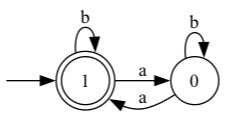
\includegraphics[width=6.5cm]{figures/even_a.png}
	\caption{The solution DFA machine to capture a string that has an even number of a's.}
	\label{fig:even_a}
\end{figure}

\section{LLM Results}

\indent\indent Developing an effective prompt for LLMs to generate regex using only the standard set of operators proved to be an iterative and somewhat delicate process. One of the persistent challenges was conveying that the input alphabet consisted solely of the characters $a$ and $b$. Despite multiple prompt refinements, the model frequently interpreted this constraint as a directive to use the explicit disjunction $(a|b)$, rather than the shorthand $.$ to represent any character within the defined alphabet. This behavior reflects a broader limitation of LLMs: they lack a formal understanding of semantic equivalence. In this case, they fail to recognize that $.$ and $(a|b)$ are functionally identical under a fixed alphabet.

\indent\indent Another issue surfaced as the prompt history grew longer. Initially, the system prompt reliably constrained the model to use only standard regex operators. However, as additional benchmark prompts were introduced in sequence, the model began to drift from the original specification. Around benchmark 12, responses increasingly violated earlier constraints, suggesting that the LLM was "forgetting" the original instructions. This degradation highlights a fundamental limitation in prompt-based control: when engaging with LLMs interactively over extended sequences, it becomes difficult to maintain consistency, especially when relying solely on static system prompts.

\indent\indent The model's reasoning style evolved over two sets of conversations. For the initial set of benchmarks (1-11), it generated one-shot answers—regex expressions without any accompanying explanation. These outputs were all correct and closely matched (or even exactly replicated) the manually written regex solutions, suggesting the model was likely retrieving or reconstructing familiar patterns from its training data. However, starting with benchmark 12 in a new conversation--—without system-level reminders or reissued constraints--—the model shifted its approach. It began breaking down the prompt into logical steps, reasoning through the requirements before proposing a solution. This reasoning-based approach yielded correct results for benchmarks 13, 17, and 22. However, these solutions often relied on enumerating all possible cases that satisfied the requirements, resembling a verbose switch-case structure in program synthesis. While functional, this approach lacks elegance and can hinder readability and maintainability.

\indent\indent One hypothesis is that the increased complexity of benchmark 12 prompted this behavioral shift. Once the model encountered a problem that didn't map cleanly onto a memorized pattern, it defaulted to reasoning. While sometimes helpful, this strategy proved less effective for simpler problems, where direct pattern recognition would have sufficed. As the benchmarks continued to grow in difficulty—particularly those involving negation or constraints requiring implicit counting—the model increasingly produced incorrect regex. Notably, it struggled with counting constructs, often failing to distinguish between mandatory and optional repetitions. For example, in attempting to describe "at least three $a$'s," it returned $aaa*$ instead of the correct $aaaa*$, mistakenly treating the third $a$ as optional.

\indent\indent Overall, the LLM's early success with one-shot outputs correlated strongly with benchmark tasks that were simple and structurally familiar. As task complexity increased, the model's shift toward reasoning introduced more nuanced errors, often stemming from overgeneralization or misinterpretation of constraints. Nonetheless, even when incorrect, the outputs frequently resembled the structure of a valid solution—indicating that the model had some abstract grasp of the form, even if the details were flawed. These results reinforce the broader theme that LLMs excel at recalling surface-level patterns from training but falter under compositional reasoning, especially in domains that demand formal correctness.


\begin{quote}
    This GPT takes a structured prompt consisting of a natural language description, a list of positive string examples, and a list of negative string examples. The format is: a one-line description, followed by '+++', then one or more positive examples, followed by '---', then one or more negative examples. Based on this, it generates a minimal theoretical regular expression using only the operations of concatenation, union, Kleene star, and the wildcard symbol '.'. It ensures that the generated expression accepts all positive examples and rejects all negative examples. The '?' symbol may be used to denote either a term or the empty language, when necessary. The alphabet is limited to 'a' and 'b', and the character 'X' in any input stands for a wildcard representing either 'a' or 'b'. When the output regex needs to match either 'a' or 'b', it uses '.' instead of '(a|b)' for minimality.
\end{quote}

\begin{table}[h!]
	\centering
	\caption{The results of the benchmarks synthesized by GPT-4o, demonstrating the performance of the LLM in generating regular expressions.}
	\label{tab:llm_outputs}
	\begin{tabular}{|c|l|l|l|}
	\hline
	\textbf{No} & \textbf{Description} & \textbf{Output} & \textbf{Correct?} \\
	\hline
	1 & Starts with a & $a.*$ & \tikzcmark \\
	2 & Ends with ab & $.*ab$ & \tikzcmark \\
	3 & Contains the substring abab & $.*abab.*$ & \tikzcmark \\
	4 & Begins with b and ends with a & $b.*a$ & \tikzcmark \\
	5 & Length is at least 3 and the 3rd symbol is a & $..a.*$ & \tikzcmark \\
	6 & Length is a multiple of 3 & $(...)*$ & \tikzcmark \\
	7 & Number of a's is divisible by 3 & $(b*ab*ab*ab*)*b*$ & \tikzcmark \\
	8 & Even number of a's & $(b*ab*ab*)*b*$ & \tikzcmark \\
	9 & Fifth symbol from the right is b & $.*b....$ & \tikzcmark \\
	10 & Alternating a and b & $(ab)*(a)?|(ba)*(b)?$ & \tikzcmark \\
	11 & Each a in w is followed by at least one b & $(b|ba)*$ & \tikzcmark \\
	12 & a$^n$b$^m$ where $n \geq 3$ and $m$ is even. & $aaa.*(bb)*$ & \tikzxmark \\
	13 & Have at most two a's & $b*|b*ab*|b*ab*ab*$ & \tikzcmark \\
	14 & Starting a and odd length or b and even length & $a(..)* | b(..)*$ & \tikzxmark \\
	15 & Length greater than 1 & $..*$ & \tikzxmark \\
	16 & Does not end with ab & $?|.|.*(aa|ba|bb)$ & \tikzxmark \\
	17 & Contain at least one a and at most one b & $aa*|aa*ba*|a*baa*$ & \tikzcmark \\
	18 & At least two b between any two a & $b*a(bb*a)*b*$ & \tikzxmark \\
	19 & Does not contain baa & $(aa|ab|ba?|bb)*a?$ & \tikzxmark \\
	20 & Every odd position is b & $(b.)*b?$ & \tikzcmark \\
	21 & Consecutive pair aa appears exactly once & $(b|ab)*aa(b|ab)*$ & \tikzxmark \\
	22 & Length $\ge 2$ and does not end with ba & $.*(aa|bb|ab)$ & \tikzcmark \\
	23 & Even a's, each a is followed by at least one b & $b*(abb*abb*)*b*$ & \tikzcmark \\
	24 & All adjacent a's appear before any adjacent b's & $(a|ba)*(bb(a|b)*a?b*)?$ & \tikzxmark \\
	25 & At most one pair of consecutive b's & $(a|ba)* | (a|ba)*bb(a|ba)*$ & \tikzxmark \\
	\hline
\end{tabular}
\end{table}

\indent\indent Upon reviewing the results in Table~\ref{tab:llm_outputs}, we observe that for benchmarks 1 through 6, as well as benchmark 9, the LLM-generated regex expressions exactly match the manually authored ground truth. These examples represent problems where the target expression is relatively simple and where only a single minimal and semantically clean regex is likely. The convergence between the LLM output and the human-written regex in these cases suggests that the model is not just generating plausible-looking patterns, but also capturing the underlying structure when it aligns well with common training examples.

\indent\indent For benchmarks 7 and 8, the model produced correct and valid solutions, such as $(b*ab*ab*ab*)*b*$ for benchmark 7. While semantically accurate, these expressions are longer than necessary and could be simplified. However, the verbosity in these outputs arguably improves readability by making the intended repetitions more explicit. In contrast, the ground truth prioritizes minimal string length, often at the cost of visual clarity. This discrepancy raises an interesting point: readability and brevity do not always align, and models trained on human-written code may favor explicit enumeration over abstraction.

\indent\indent Benchmark 10 highlights a situation where the LLM unnecessarily introduces a union to distinguish between inputs beginning with a or b. Although the result is functionally correct, the added complexity neither enhances correctness nor readability, and it contrasts with the simpler expected solution. In benchmark 11, despite its slightly increased complexity, the model again matched the correct regex exactly.

\indent\indent From benchmark 12 onward, the correctness rate declines. Benchmark 12 is incorrect because it allows for an odd number of b characters, violating the requirement that bs appear in even counts. Benchmarks 13 and 17, while correct in behavior, exhibit syntactic redundancy that could be removed with minor simplification. For example, patterns with nested repetitions or excessive alternations can often be flattened without affecting correctness.

\indent\indent Benchmarks 14, 15, and 18 all display a common off-by-one counting error—a recurring failure mode for LLMs in tasks that involve precise cardinality constraints. These errors reveal the model's difficulty in reasoning about exact quantities, a known limitation in sequence modeling.

\indent\indent Benchmark 16 contains invalid regex syntax, misusing the ? operator without a preceding token. The intended goal may have been to include optional content, but the structure used violates standard regex grammar. Similarly, benchmark 19 is logically flawed: the use of $(aa|ab|ba?|bb)*$ followed by a suffix expression can incorrectly accept strings like bbaa, which should be rejected. This occurs because of incorrect assumptions about how the starred term interacts with the rest of the expression.

\indent\indent In contrast, benchmark 20 is entirely correct, demonstrating that the model can occasionally capture subtle constraints when the structure of the problem is well-aligned with common representations. However, benchmark 21 fails due to overpermissiveness. The pattern $aa(b|ab)*$ accepts strings like aaab, which includes two pairs of consecutive as—violating the task specification.

\indent\indent Benchmark 22 is nearly correct, but misses a boundary case: it fails to handle strings with fewer than two characters, which should automatically satisfy the negated condition of “not ending in ba.” Benchmark 23 is both correct and highly human-readable, though there are opportunities for syntactic reduction, such as eliminating unnecessary $b*$ terms in the suffix. This speaks again to the tension between brevity and expressiveness.

\indent\indent Finally, benchmarks 24 and 25 are incorrect due to subtle logic flaws. In 24, the use of $(a|b)*$ is too permissive and allows the occurrence of double a after bb, violating the restriction. In 25, the model allows bbba via $bb(a|ba)*$, a construction that does not correctly constrain repetition patterns involving pairs of bs.

\indent\indent Overall, the model's strongest performance appears in problems that are well-aligned with familiar symbolic patterns, especially those involving prefixes, suffixes, or fixed-length structural constraints. As tasks begin to involve negation, exact counting, or nested disjunctions, correctness degrades. Notably, even incorrect outputs often resemble the correct structure, suggesting that the model maintains a surface-level understanding of the domain—but without the formal rigor needed for correctness in all cases.

\section{Integration Synthesis}

\subsection{LLM and AlphaRegex Integration}
\indent\indent We explored the potential of integrating LLMs with AlphaRegex to enhance regex synthesis. The idea was to leverage the strengths of both approaches: the LLM's ability to generate human-readable regex and AlphaRegex's efficiency in synthesizing correct solutions.

\indent\indent Though not fully implemented, we explored ideas for combining models. One early prototype used ChatGPT to generate candidate regex, which were validated and refined by AlphaRegex. This semi-automated pipeline showed promise: even when the LLM failed to produce correct output directly, its regex often seeded AlphaRegex with promising starting points. The particular regex generated by ChatGPT can be incorrect, we can construct the regex in the internal representation of AlphaRegex, and then run the synthesis algorithm to find a solution. This approach can be seen as a hybrid model that leverages the strengths of both LLMs and traditional synthesis methods. 

\subsection{LLM and L* Integration}
\indent\indent Another promising approach involves leveraging ChatGPT to generate Python test cases for verifying the correctness of regex solutions. By providing the natural language description and examples as input, ChatGPT can output Python code that automates the validation process. This approach significantly reduces the manual effort required for constructing membership and equivalence queries in the L* algorithm.
\indent\indent For instance, for benchmark 14, which is a challenging example, we can use an LLM to automate the membership queries. The task involves checking if the first character is 'a' and the length is odd, or if the first character is 'b' and the length is even. ChatGPT can generate Python code like the following:

\begin{verbatim}
if w[0] == 'a' and len(w) % 2 == 1:
    return True
if w[0] == 'b' and len(w) % 2 == 0:
    return True
return False
\end{verbatim}

\indent\indent This Python code can then be used to act as a large art of the MAT answering the membership queries generated by the L* algorithm. By automating the verification process, this approach streamlines the synthesis pipeline and ensures consistency in evaluating correctness.

\subsection{AlphaRegex and L* Integration}
\indent\indent The integration of AlphaRegex and L* is another promising avenue for future work. By combining the strengths of both methods, we can potentially improve the synthesis process. For example, L* could serve as a guide to generate high-quality examples that AlphaRegex can use to refine its search. This hybrid approach could leverage L*'s ability to systematically explore the space of possible solutions while benefiting from AlphaRegex's heuristics to efficiently navigate the search space.

\indent\indent The integration of these two methods could also address some of the limitations observed in their individual performances. For instance, AlphaRegex's challenges with union operations could be mitigated by L*'s structured generation of counterexamples, which can help AlphaRegex focus on critical areas of the search space. Conversely, AlphaRegex's heuristics could enhance L*'s exploration by providing initial candidates or pruning less promising paths, thereby reducing the number of membership and equivalence queries required.

\section{Discussion}

\subsection{Lessons for Broader Synthesis}
\indent\indent The findings from our results provide several insights that can generalize to other program synthesis tasks. The effectiveness of heuristics in reducing the search space, as demonstrated with AlphaRegex, underscores the importance of carefully designed heuristics in program synthesis. However, it is crucial to balance the trade-off between computational overhead and the reduction of the search space. The performance of LLMs highlights the significance of structured and well-defined input representations. By providing clear examples and constraints, synthesis models can be guided to generate more accurate outputs. The integration of LLMs with traditional synthesis methods suggests that hybrid approaches can leverage the strengths of different paradigms. For example, LLMs can offer initial guesses or templates, while formal methods refine and validate the solutions.

\indent\indent The multi-faceted evaluation metrics used in this study—correctness, efficiency, and complexity—are broadly applicable to other synthesis tasks, ensuring a holistic assessment of synthesized programs. Observing failure cases, such as the inability of AlphaRegex to handle unions effectively, emphasizes the importance of analyzing and addressing specific limitations in synthesis algorithms. The reliance on human interpretation for L* algorithm inputs and the qualitative analysis of regex readability highlight the value of human-in-the-loop systems for complex synthesis tasks. Furthermore, the time and state exploration results emphasize the need for scalable algorithms, especially as problem complexity increases. Techniques like pruning and approximation can be adapted to address scalability challenges in other domains.

\indent\indent The tendency of LLMs to overfit to examples illustrates the broader challenge of balancing generalization and specificity in program synthesis. These lessons suggest that combining domain-specific insights, robust evaluation frameworks, and hybrid methodologies can enhance the applicability and effectiveness of program synthesis across diverse domains.

\indent\indent These lessons suggest that combining domain-specific insights, robust evaluation frameworks, and hybrid methodologies can enhance the applicability and effectiveness of program synthesis across diverse domains.

\vspace{2em}

